% !TeX encoding = utf-8
% !TeX program = pdflatex
% !Mode:: "TeX:UTF-8"
% =============================================================
% 2026 第十二届数维杯（秋季赛）英文赛道论文骨架
% 版式：官方 swmcmthesis.cls v1.8（LaTeXStudio，2026/11/06）
% 编译：.\build.ps1 -Target en      （pdflatex ×3，无需 bibtex）
% 赛时只改正文；红色 [PLACEHOLDER] 是必须替换的内容位
% =============================================================
\documentclass{swmcmthesis}

% ---- 官方类未加载、本文骨架需要的宏包 ----
% 类已加载：amsmath/amssymb/bm、graphicx、booktabs、longtable、multirow、
%           array、lastpage、caption、enumitem、listings、subfigure、
%           pdfpages、cleveref、hyperref、newtxtext/newtxmath、lipsum、mwe
\usepackage{tikz}
\usetikzlibrary{arrows.meta,positioning}
\usepackage[ruled,vlined,linesnumbered]{algorithm2e}
\usepackage{siunitx}
\sisetup{detect-all, group-separator={,}}

\newcommand{\ph}[1]{{\color{red}[#1]}}   % 红色占位；交稿前清零

%%%%%%%%%%%% 填写相关信息 %%%%%%%%%%%%%%%%%%%%%%%%%%
\title{\ph{Model Title: A Concise, Claim-Shaped Name}}  % 论文题目

\baominghao{SWBMCM2600001}   % 报名号/队号：换成自己的
\zubie{C}                    % 选题：A / B / C
\date{2026}                  % 年份（封面中间那行）

\abstract{%
[Summary recipe --- graders may read only this page. Paragraph 1: the problem
and the goal. Paragraph 2: what model you built, what the variables and
constraints are. Paragraph 3: how you solved it. Paragraph 4: three findings,
each carrying a concrete number. Final sentence: the value and the boundary of
the model. 400--600 words, no equations, no citations.]

This paper addresses [problem statement in one clause]. We develop a
[model family] that couples [component A] with [component B], and we solve it
by [method]. Three findings follow. First, [finding 1 with a number]. Second,
[finding 2 with a number]. Third, [finding 3 with a number]. The model is
validated against [baseline] and stays stable under [perturbation], which
supports [decision implication].
}

\keywords{mathematical modeling; [keyword 2]; [keyword 3]; sensitivity analysis}

\begin{document}

\maketitle          % 生成 Summary Sheet（首页）
\tableofcontents    % 目录

\newpage
\setcounter{page}{1}

% ============================ 1 Introduction ============================
\section{Introduction}

\subsection{Problem Background}
[Three to five paragraphs: background, current practice, the gap in that
practice, and therefore the model that closes the gap. One idea per paragraph;
let each paragraph end on the sentence that opens the next.]

\subsection{Restatement of the Problem}
We are asked to [\textbf{(i)} ...], [\textbf{(ii)} ...], and
[\textbf{(iii)} ...]. Formally, given [input], determine [output] such that
[constraint], while optimizing [objective].

\subsection{Our Work}
The contributions are summarized as follows.
\begin{enumerate}
  \item A [model name] that [makes what explicit].
  \item A [solver] that reduces the computation from [order] to [order].
  \item An evaluation on [data] showing [headline number].
\end{enumerate}

% ============================ 2 Assumptions ============================
\section{Assumptions and Symbol Description}

\subsection{Assumptions}
\begin{enumerate}
  \item \textbf{[Assumption statement.]} [Why it is acceptable, and what breaks
        if it fails.]
  \item \textbf{[Assumption statement.]} [Justification with a citation or a
        dimensional argument.]
  \item \textbf{[Assumption statement.]} [Justification.]
\end{enumerate}

\subsection{Symbol Description}
\begin{table}[!h]
\centering
\caption{Main notations.}
\label{tab:notation}
\begin{tabular}{lll}
\toprule[1.5pt]
Symbol & Description & Unit \\
\midrule[1pt]
$x_{i}$        & [decision variable]      & m \\
$c_{ij}$       & [cost coefficient]       & CNY \\
$\theta$       & [model parameter]        & -- \\
$J(\cdot)$     & objective functional     & -- \\
\bottomrule[1.5pt]
\end{tabular}
\end{table}

% ============================ 3 Model ============================
\section{Model Development}

\subsection{Formulation}
Let $\mathcal{I}$ be the set of [items]. The decision is
\begin{equation}
  \min_{x}\; J(x)=\sum_{i\in\mathcal{I}} c_{i}x_{i}
      +\lambda\sum_{i<j} w_{ij}\,\lvert x_{i}-x_{j}\rvert ,
  \label{eq:obj}
\end{equation}
subject to
\begin{align}
  \sum_{i\in\mathcal{I}} a_{i}x_{i} &\le b, \label{eq:cap}\\
  x_{i} &\ge 0,\quad x_{i}\in\mathbb{Z}\ \text{for}\ i\in\mathcal{I}_{d},
  \label{eq:int}
\end{align}
where $\lambda\ge 0$ trades efficiency against [equity], and \eqref{eq:cap}
encodes [the binding resource]. The relaxation of \eqref{eq:int} follows the
standard convex treatment.

\subsection{Solution Framework}
Figure~\ref{fig:pipeline} shows the four stages of the pipeline.

\begin{figure}[!ht]
  \centering
  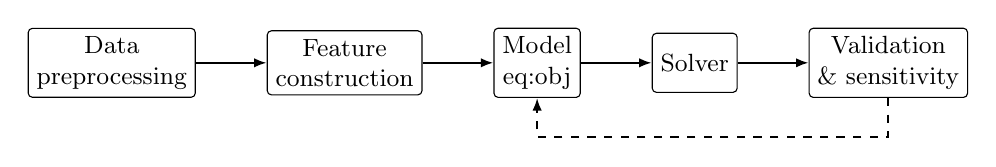
\begin{tikzpicture}[
      node distance=6mm and 9mm,
      box/.style={draw, rounded corners=1.5pt, align=center,
                  minimum height=7.5mm, inner sep=3pt, font=\small},
      ar/.style={-{Latex[length=1.6mm]}, thick}]
    \node[box] (d)  {Data\\preprocessing};
    \node[box, right=of d]  (f) {Feature\\construction};
    \node[box, right=of f]  (m) {Model\\\eqref{eq:obj}};
    \node[box, right=of m]  (s) {Solver};
    \node[box, right=of s]  (v) {Validation\\\& sensitivity};
    \draw[ar] (d) -- (f);
    \draw[ar] (f) -- (m);
    \draw[ar] (m) -- (s);
    \draw[ar] (s) -- (v);
    \draw[ar, dashed] (v.south) -- ++(0,-5mm) -| (m.south);
  \end{tikzpicture}
  \caption{Solution pipeline. [Every figure must be cited in the text and
  explained in one sentence.]}
  \label{fig:pipeline}
\end{figure}

\begin{algorithm}[!ht]
  \caption{Hybrid search for \eqref{eq:obj}}\label{alg:solve}
  \KwIn{instance $\mathcal{I}$, budget $b$, population $N$, generations $G$}
  \KwOut{best feasible $x^{*}$}
  initialize population $\mathcal{P}\leftarrow\{x^{(1)},\dots,x^{(N)}\}$\;
  \For{$g=1$ \KwTo $G$}{
    evaluate $J$ by \eqref{eq:obj} under \eqref{eq:cap}--\eqref{eq:int}\;
    select parents by tournament; apply crossover and mutation\;
    repair infeasible offspring by [repair rule]\;
  }
  \Return{$\arg\min_{x\in\mathcal{P}} J(x)$}\;
\end{algorithm}

% ============================ 4 Results ============================
\section{Results and Analysis}

\subsection{Main Results}
Table~\ref{tab:main} reports the comparison against [baseline].

\begin{table}[!ht]
\centering
\caption{Performance on [dataset / scenario].}
\label{tab:main}
\begin{tabular}{lccc}
\toprule[1.5pt]
Method & Metric 1 & Metric 2 & Time (s) \\
\midrule[1pt]
Baseline           & 12.400 & 0.910 & 8.2 \\
{[Ours (v1)]}      & 15.700 & 0.945 & 6.4 \\
{[Ours (full)]}    & 18.300 & 0.968 & 4.9 \\
\bottomrule[1.5pt]
\end{tabular}
\end{table}

\begin{figure}[!ht]
  \centering
  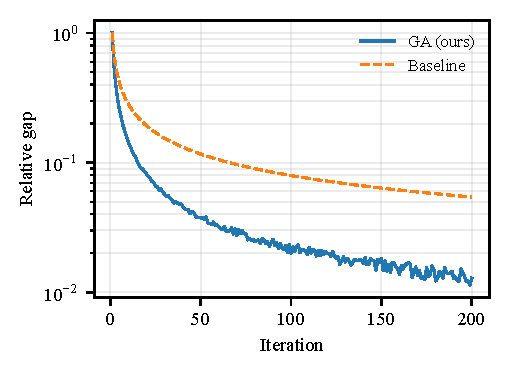
\includegraphics[width=0.62\textwidth]{figures/fig_convergence.pdf}
  \caption{Convergence of the proposed solver ([replace with real results]).}
  \label{fig:conv}
\end{figure}

\subsection{Discussion}
[Do not restate the table. Each paragraph answers one question: why is it
faster, where does the gain come from, and what does it cost. Explain the
mechanism in because-clauses instead of writing that the result is good.]

% ============================ 5 Sensitivity ============================
\section{Sensitivity Analysis}
We perturb $\theta$ over [range] and re-solve. Figure~\ref{fig:sens} shows that
the objective changes by [x\%] before [the ranking flips], which means the
recommendation is [robust / fragile] within [practical range].

\begin{figure}[!ht]
  \centering
  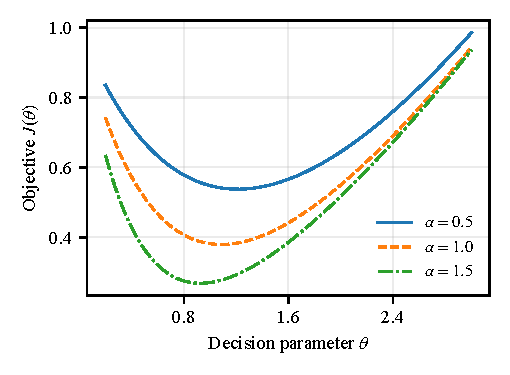
\includegraphics[width=0.62\textwidth]{figures/fig_sensitivity.pdf}
  \caption{Objective versus decision parameter ([replace with real results]).}
  \label{fig:sens}
\end{figure}

% ============================ 6 Evaluation ============================
\section{Strengths and Weakness}

\subsection{Strengths}
\begin{itemize}
  \item {[Strength tied to a result, not to an adjective.]}
  \item {[Strength tied to generality or interpretability.]}
\end{itemize}

\subsection{Weakness and Extensions}
\begin{itemize}
  \item {[Limitation, plus the concrete extension that removes it.]}
\end{itemize}

% ============================ 7 Conclusion ============================
\section{Conclusion}
[Four to six sentences: return to the question, state the final numeric
conclusion, and mark the boundary of applicability. Introduce nothing new.]

% ============================ References ============================
\begin{thebibliography}{9}
\bibitem{bib:deb2002}
K. Deb, A. Pratap, S. Agarwal and T. Meyarivan, A fast and elitist
multiobjective genetic algorithm: NSGA-II, \textit{IEEE Transactions on
Evolutionary Computation}, 2002, 6(2): 182--197.

\bibitem{bib:huangfu2018}
Q. Huangfu and J. A. J. Hall, Parallelizing the dual revised simplex method,
\textit{Mathematical Programming Computation}, 2018, 10(1): 119--142.

\bibitem{bib:saltelli2008}
A. Saltelli, M. Ratto, T. Andres, F. Campolongo, J. Cariboni, D. Gatelli,
M. Saisana and S. Tarantola, \textit{Global Sensitivity Analysis: The Primer},
Chichester: John Wiley \& Sons, 2008.

\bibitem{bib:boyd2004}
S. Boyd and L. Vandenberghe, \textit{Convex Optimization}, Cambridge: Cambridge
University Press, 2004.
\end{thebibliography}

% ============================ Appendix ============================
\newpage
\section*{Appendix}
\addcontentsline{toc}{section}{Appendix}

% 版式注意：numbers=left 会把行号排到版心左侧外面，frame=single 的左右竖线也会外扩
% 约 4pt，两者都会被投稿前检查判成「冲出栏宽」。xleftmargin 把正文框整体右移，
% 让行号落回版心内；frame=tb 与官方 cls 默认一致，只画上下横线，不产生竖向溢出。
\lstset{basicstyle=\small\ttfamily, breaklines=true, frame=tb,
        numbers=left, numberstyle=\tiny, xleftmargin=2.5em,
        keywordstyle=\color{blue}, commentstyle=\color{dkgreen}}

\begin{lstlisting}[language=Python,caption={Solver core (excerpt).}]
import numpy as np
from scipy.optimize import milp, LinearConstraint, Bounds

def solve(c, A, b, integer_mask):
    """Solve min c^T x  s.t.  A x <= b, x >= 0, integrality on mask."""
    res = milp(c=c,
               constraints=LinearConstraint(A, -np.inf, b),
               integrality=integer_mask.astype(int),
               bounds=Bounds(0, np.inf))
    return res.x, res.fun
\end{lstlisting}

\end{document}
